\section{Introducci\'on}

En el presente trabajo se aborda el problema de segmentaci\'on de im\'agenes: dada una imagen buscamos obtener una partici\'on de esta donde cada regi\'on delimitada represente un objeto identificable y distinguible. Claramente este no es un problema bien definido, ya que depende de la percepci\'on subjetiva de cada individuo sobre que es lo que se puede observar en una imagen espec\'ifica. Debido a esto es com\'un que distintos trabajos busquen dar soluciones a conjuntos de fotos sobre un área determinada, como por ejemplo im\'agenes m\'edicas para el estudio de tumores en el cerebro, aprovechando características especiales del objeto de estudio. \\

\begin{figure}[H]
	\begin{center}
		\subfigure[Imagen original]{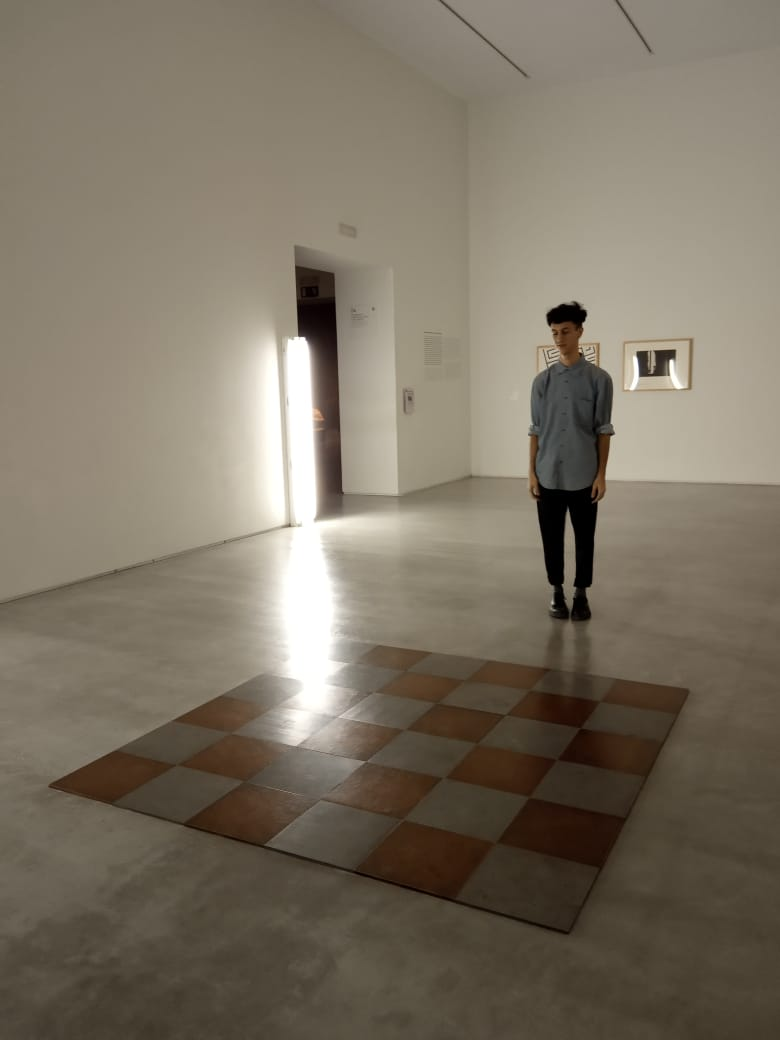
\includegraphics[height=208pt, width=156pt]{segmentaciones/museo.jpg}}
		\subfigure[Segmentaci\'on generada ($k=12500$)]{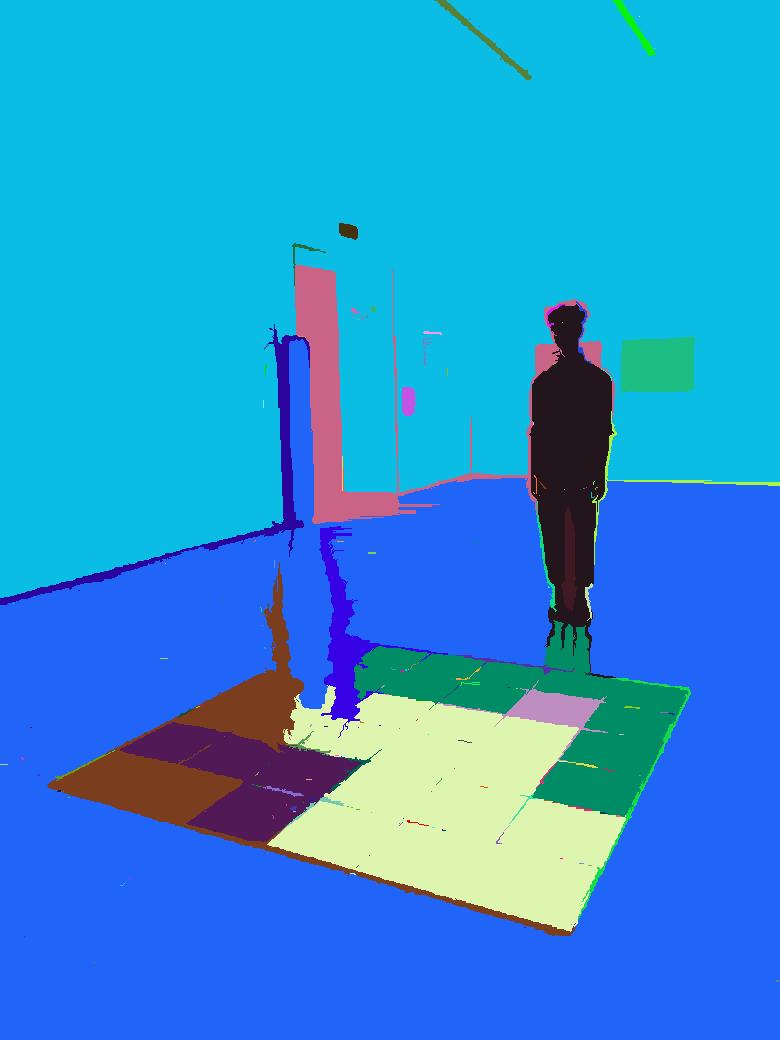
\includegraphics[height=208pt, width=156pt]{segmentaciones/museo_seg.jpg}}
	\end{center}
	\caption{Ejemplo de una segmentaci\'on}
	\label{ejemplo}
\end{figure} 

Se puede observar en la figura \ref{ejemplo} que si bien se logran distinguir las partes centrales de la im\'agen (persona, cuadrados, cuadros, pared, piso) en la imagen original pueden haber muchos factores que influencian de manera negativa en la separaci\'on. Un claro ejemplo es la luz de tubo junto a la puerta que impacta notablemente sobre el piso, o la sombra del sujeto afectando sobre los cuadrados. Al mismo tiempo, como se explicara m\'as adelante, buscar una segmentaci\'on muy general puede perder detalles que podr\'ian ser interesantes, como las distinciones entre cuadrados dentro del cuadrado principal en el piso.\\ 
Para la resoluci\'on del problema, el trabajo se basa en el m\'etodo expuesto por Pedro F. Felzenszwalb y Daniel P. Huttenlocher \cite{Felzenszwalb2004} que, como describiremos en las secciones siguientes, proponen un algoritmo eficiente basado en grafos para conseguir una segmentaci\'on ``ni muy fina ni muy gruesa'' en su terminolog\'ia. A lo largo del trabajo se estudia este m\'etodo en profundidad, considerando las distintas implementaciones posibles, midiendo la eficiencia de estas e intentando responder a la pregunta de si el predicado propuesto por Felzenszwalb y Huttenlocher verdaderamente se refleja en los resultados obtenidos.

